\documentclass[unpublished]{btswhitepaper}
\title{BitShares 2.0: General Overview}
\author{
 \IEEEauthorblockN{Fabian~Schuh}
 \IEEEauthorblockA{BitShares Europe, BitShares.eu\\
                   Erlangen, Germany\\
                   Email: \texttt{fabian@bitshares.eu}}
 \and
 \IEEEauthorblockN{Daniel~Larimer}
 \IEEEauthorblockA{Cryptonomex, Cryptonomex.com\\
                   Blacksburg (VA), USA\\
                   Email: \texttt{dan@cryptonomex.com}}%
 \thanks{This work was supported by Cryptonomex and honorable members of the
         bitsharestalk.org community.}
}

\begin{document}
\maketitle

\begin{abstract}%
 BitShares 2.0 is an industrial-grade decentralized platform built for
 high-performance financial smart contracts. The decentralized exchange that
 allows for trading of arbitrary pairs without counterparty risk facilitates
 only one out of many available features. Market-pegged assets, such as the
 bitUSD, are crypto tokens that come with all the advantages of traditional
 cryptocurrencies like bitcoin but trade for at least the value of their
 underlying asset, e.g. \$1. Furthermore, BitShares represents the first
 decentralized autonomous company that lets its shareholders decide on its
 future direction and products. This paper gives a brief overview over the
 whole BitShares platform, recapitulates known blockchain technologies and
 redefines \emph{state-of-the-art}.
\end{abstract}

\section       { Introduction                      } BitShares is a technology supported by next generation entrepreneurs,
investors, and developers with a common interest in finding free market
solutions by leveraging the power of globally decentralized consensus and
decision making. Consensus technology has the power to do for economics what
the internet did for information. It can harness the combined power of all
humanity to coordinate the discovery and aggregation of real-time knowledge,
previously unobtainable. This knowledge can be used to more effectively
coordinate the allocation of resources toward their most productive and
valuable use.

Bitcoin is the first fully autonomous system to utilize distributed consensus
technology to create a more efficient and reliable global payment network. The
core innovation of Bitcoin is the Blockchain, a cryptographically secured
public ledger of all accounts on the Bitcoin network that facilitates the
transfer of value from one individual directly to another. For the first time
in history, financial transactions over the internet no longer require a middle
man to act as a trustworthy, confidential fiduciary.

BitShares looks to extend the innovation of the blockchain to more industries
that rely upon the internet to provide their services. Whether its banking,
stock exchanges~\cite{btst:oldwp}, lotteries~\cite{play}, voting~\cite{fmv},
music~\cite{peertracks}, auctions or many
others, a digital public ledger allows for the creation of \emph{distributed
autonomous companies} (or DACs) that provide better quality services at a
fraction of the cost incurred by their more traditional, centralized
counterparts. The advent of DACs ushers in a new paradigm in organizational
structure in which companies can run without any human management and under the
control of an incorruptible set of business rules. These rules are encoded in
publicly auditable open source software distributed across the computers of the
companies' shareholders, who effortlessly secure the company from arbitrary
control.

BitShares does for business what bitcoin did for money by utilizing distributed
consensus technology to create companies that are inherently global,
transparent, trustworthy, efficient and most importantly profitable. Why and
how BitShares achieves a decentralized but profitable business is described in
more detail in a distinct paper~\cite{}. % FIXME business plan paper

BitShares has went through many changes and has done its best to stay on top of
blockchain technology. Towards the end of 2014 some of the DACs were merged and
the X was dropped from "BitShares X" to become simply BitShares (BTS).

The next step in the evolution of BitShares was named \emph{Bitshares 2.0}, and
incorporates all of the feedback and lessons learned from the BitShares
stakeholders, partners, developers, marketers, and other community leaders
throughout a full year of research and development.

With the former BitShares 1.0, the core development team has closely controlled
the development and direction of BitShares. With BitShares reaching maturity at
version 2.0, the team is ready to remove the training wheels, and let the
direction of all future development be decided completely by stakeholder vote.

By utilizing a new worker voting system that will be included in BitShares 2.0,
the development will continue in whatever direction is approved by its
stakeholders. With this new structure, BitShares will be more robust, and
sustainable while being agile, flexible and adaptive to overcome unforeseen
hurdles of the future.

This paper is intended as an introduction to BitShares 2.0 and presents the
basic concepts of the peer-to-peer nature, the distributed public ledger in
form of a blockchain, and give a brief overview of the decentral consensus
mechanism applied to reach blockchain state consensus. We further discuss the
basic blockchain tokens (BTS), its distribution and usage in BitShares. We
also describe the wallet and operations with the network as well as outline the
functionalities of BitShares accounts.
 

\section       { Base Token                        } In the BitShares network the base token is called \emph{a BitShare} and carries
the abbreviation \texttt{BTS}. It is dividable into $10^5$ sub-units which are
denoted as follows:
\begin{align*}
\SI{1}{mises } &= \SI{0.00001}{BTS}\\
\SI{1}{xennon} &= \SI{0.0001}{BTS}\\
\SI{1}{oxyd  } &= \SI{0.001}{BTS}\\
\SI{1}{graphn} &= \SI{0.01}{BTS}\\
\SI{1}{epox  } &= \SI{0.1}{BTS}
\end{align*}

In general, all properties of Bitcoin also apply to BTS, namely, they have
value, can be transfered on the blockchain and are secured by elliptic curve
signatures.

In contrast to most cryptocurrencies, BitShares does not claim to be a currency
but rather equity in a decentral autonomous company (DAC). As a result, the
market valuation of BitShares is free floating and may be as volatile as any
other equity (e.g. of traditional companies).

Nonetheless, BTS tokens can be used as \emph{collateral} in financial smart
contracts~\cite{bts:financial} such as market pegged assets.

% FIXME what else?
 
\subsection    { Distribution of BTS               } BitShares has set an example of a \emph{social agreement} by establishing its
own \emph{sharedropping} standards. The idea behind sharedropping is that any
future chain will always benefit by choosing to align itself with the ones who
worked hard at making the technology possible.

Hence, the seed allocation (initial distribution) of BitShares, which took
place over a 1 year period, from November 2013 to November 2014, was achieved
by sharedropping 47\% to BitShares PTS and another 47\% to BitShares AGS.
%
This way, the full, fairness was defined by equal opportunity and in the case
of BTS we have distributed \emph{fairly} by CPU mining of PTS while,
alternatively, everyone had an additional equal opportunity by contribute to
AGS~\cite{}.

The other 6\% are set aside to secure the future of BitShares and funds its
development. However, in contrast to many other cryptocurrencies, every
shareholder has a say as to who these funds are spend (see
\cref{sec:token:supply}).

The base tokens of BitShares \emph{2.0} will be distributed on a 1:1 basis
fully honoring the BTS tokens in the BitShares \emph{1.0} network.  For the
sake of completeness, the following paragraphs will describe the initial
distribution of BTS tokens in the aforementioned BitShares 1.0 network.

The following will discuss PTS and AGS in more detail.
 
\subsubsection { Bitshares PTS                     } The original grandfather prototype formerly called proto-shares (PTS).
BitShares PTS, our \emph{prototype bitshares coin}, was a simple minable
crypto-currency (similar to Bitcoin) that was created to allow people to
advertise their interest in receiving free token samples in future DACs. PTS
functions as a high-tech \emph{mailing list} for distributing free sample
bitshares from many developers of decentral autonomous companies (DACs). The
only people who tended to own PTS tokens were those who understand DACs, so DAC
developers prefer to target them with free samples rather than \emph{air
dropping} their samples onto a much less interested general population.

The industry recommendation was that when a DAC is launched, at least 10\% of
the DAC's total tokens are given proportionally to holders of PTS. This was not
a contract or a guarantee; it was a \emph{social consensus} of those in the DAC
community about what percentage of a new DAC's tokens should be distributed to
those who have supported the BitShares industry by owning its PTS tokens.
 
\subsubsection { Bitshares AGS                     } The original grandmother prototype formerly called angel-shares (AGS) in
reference to the patron \emph{angels} who once funded the performing arts.
That's why AGS are \emph{not liquid}. (No one can trade the proof that you were
the once willing to donate to this cause.) 

The donations have been recorded in the public blockchain of bitcoin which now
acts as a \emph{book of honorable donors}. The bitcoin address used as donation
address was 
\begin{center}
 \texttt{1ANGELwQwWxMmbdaSWhWLqBEtPTkWb8uDc}
\end{center}
Note, that the donation period for AGS lasting 200 days has ended already and
that donations to this address never resulted nor will result in any
obligations whatsoever.

\bigskip

%% BTS Genesis
Having attracted two different groups of investors with a mined crypto token
via PTS and a donation based book of donors via AGS, everyone had a chance to
participate and be rewarded with stake in the genesis block of BitShares 1.0.
This genesis block solely consisted of AGS and PTS holders on a 50\%/50\% ratio
such that the BTS tokens initially issued by this genesis can be considered
\emph{well distributed}.

%% Social consensus update
However, ever since the BitShares network has launched, the social consensus
has shifted towards \emph{sharedropping} onto holders of BTS directly instead
of PTS/AGS.
 
\subsection    { Bitshares Genesis Distribution    } We see that the seed allocation (initial distribution) of BitShares, which took
place over a 1 year period, from November 2013 to November 2014, was achieved
by sharedropping 47\% to BitShares PTS and another 47\% to BitShares AGS. This
way, the full, fairness was defined by equal opportunity and in the case of BTS
we have distributed \emph{fairly} by CPU mining of PTS while, alternatively,
everyone had an additional equal opportunity by contribute to AGS.

Having attracted two different groups of investors with a mined crypto token
via PTS and a donation based book of donors via AGS, everyone had a chance to
participate and be rewarded with stake in the genesis block of BitShares 1.0.
This genesis block solely consisted of AGS and PTS holders on a 50\%/50\% ratio
such that the BTS tokens initially issued by this genesis can be considered
\emph{well distributed}.

The other 6\% are set aside to secure the future of BitShares and funds its
development and operational costs. In practice, they are put into the so called
\emph{reserves pool} that no one has control over except the BitShares
protocol. In contrast to many other crypto-currencies, every shareholder has a
say as to how these funds are spend (see \cref{sec:bts:revenue:expenses}).
 

\section       { Business Units                    } Let us discuss the organization structure of the BitShares network when
interpreted as a company. Some of these entities are associated with a cost for
the business and need to be accounted for in profit calculations.

\subsection    { BitShares Witnesses               } In BitShares, the witnesses' job is to collect transactions, bundle them into a
block, sign the block and broadcast it to the network. They essentially are the
block producers for the underlying consensus mechanism (see
\cref{sec:consensus}).

For each successfully constructed block, a witness is payed in shares that are
taken from the limited reserves pool at a rate that is defined by the
shareholders by means of approval voting.

\subsection    { BitShares Committee               } Since Bitcoin struggled to reach a consensus about the size of their blocks,
the people in the cryptocurrency space realized that the governance of a DAC
should not be ignored. Hence, BitShares offers a tools to reach on-chain
consensus about business management decisions.

The BitShares blockchain has a set of parameters available that are subject of
shareholder approval. Shareholders can define their preferred set of parameters
and thereby create a so called \emph{committee member} or alternatively vote
for an existing committee member. The BitShares committee consists of $C$
\emph{active} committee members.

For each business parameter the protocol will calculate the difference between
up- and down-votes ($v_\text{pro}-v_\text{con}$) for each active committee
member and then take the median of the top $C$ active members:
\begin{algorithmic}
 \State // Derive active C committee members
 \For{ i : active committee members }
  \State member weight: $w[i] \gets v_\text{pro}-v_\text{con}$
 \EndFor
 \State $\text{members} \gets \Call{sort}{w}$
 \State $\text{active} \gets \text{members}[0 \to C]$

 \State // For each Parameter: derive median of active members
 \For{ parameter : parameters }
   \State $p \gets \Call{GetParameters}{\text{active}, \text{parameter}}$
   \State $x = \operatorname{sort}(p[i])$
   \State $\tilde p =\begin{cases}
                        x[\frac{C+1}{2}]                                               & C \text{ odd}\\
                        \frac {1}{2}\left(x[{\frac{C}{2}}] + x[\frac{C}{2} + 1]\right) & C \text{ even.}
           \end{cases}$
  \State $\text{parameter} \gets \tilde p$
 \EndFor
\end{algorithmic}
Since, $C$ is a parameter as any other, the shareholders decide for the size of
the committee.

The BitShares ecosystem has a set of parameters available that are subject of
shareholder approval. Initially, BitShares has the following blockchain
parameters:
%
\begin{description}[leftmargin=4em,style=nextline]
 \item[{fee structure}:        ] fess that have to be paid by costumers for individual transactions
 \item[{block interval}:       ] i.e. block interval, max size of block/transaction
 \item[{expiration parameters}:] i.e. maximum expiration interval
 \item[{witness parameters}:   ] i.e. maximum amount of witnesses (block producers)
 \item[{committee parameters}: ] i.e. maximum amount of committee members
 \item[{witness pay}:          ] payment for each witnesses per signed block
 \item[{worker budget}:        ] available budget available for budget items (e.g. development)
\end{description}
Please note that the given set of parameters serves as an example and that the
network's parameters are subject to change over time.

\medskip

Additionally to defining the parameters any active witness can propose a
protocol or business upgrade (i.e. hard fork) which can be voted on (or
against) by shareholders. When the total votes for the hard fork are greater
than the median witness weight $w$ then the hard fork takes effect.

\subsection    { BitShares Budget Items/Workers    } Thanks to the funds stored in the reserve pool, BitShares can offer to not only
pay for its own development and protocol improvement but also support and
encourage growth of an ecosystem.

In order to be get paid by BitShares, a proposal containing
\begin{inparaenum}[(a)]
 \item the date of work begin,
 \item the date of work end,
 \item a daily pay (denoted in BTS),
 \item the worker's name, and
 \item an internet address.
\end{inparaenum}
has to be publish on the blockchain and approved by shareholders.
A worker can also choose on of the following properties:
\begin{itemize}
 \item \emph{vesting}: pay to the worker's account
 \item \emph{refund}: return the pay back to the reserve pool to be used for
                      future projects
 \item \emph{burn}: destroys the pay thus reducing share supply, equivalent to
                    share buy-back of a company stock.
\end{itemize}

A blockchain parameter (defined by shareholders through the committee) defines
the daily available budget. No more than that can be paid at any time to all so
called \emph{workers} combined.

The daily budget is distributed as illustrated in \cref{fig:workerpayalgo}: 
\begin{inparaenum}[(1)]
 \item The available budget is taken out of reserves pool.
 \item The budget items are sorted according to their approval rate
       ($v_\text{pro}-v_\text{con})$ in a descending order.
 \item Starting at the worker with the highest approval rate, the requested
       daily pay is payed until the daily budget is depleted.
 \item The worker with the least approval rate that was paid may receive less
       than the requested pay
\end{inparaenum}

\begin{figure}[!htp]
 \centering
  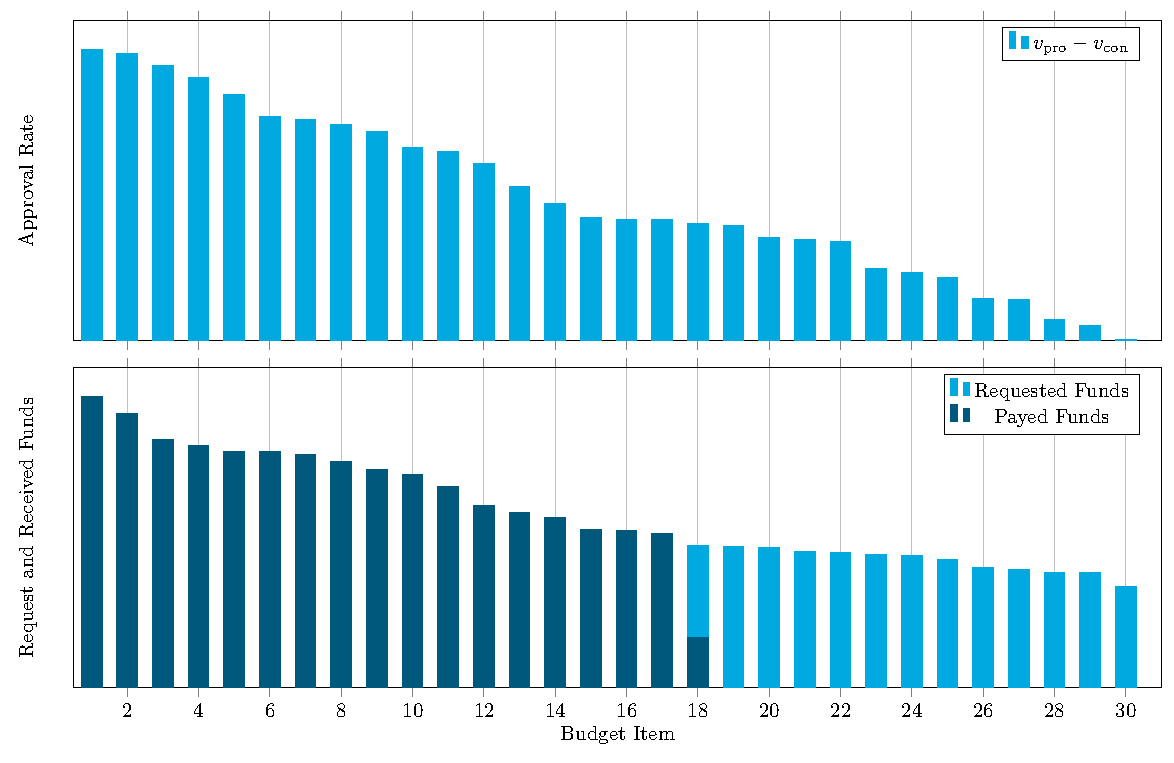
\includegraphics[width=\linewidth]{figures/worker-pay-algo.pdf}\vspace*{-2ex}
 \caption{Illustration of budget item payments.}
 \label{fig:workerpayalgo}
\end{figure}
Hence, in order to be successfully funded by the BitShares ecosystem, the
shareholder approval for your budget item needs to be highly ranked.

Since the payments for workers from the non-liquid reserve pool result in an
increased supply of BTS, these payments are vesting over a period of time
defined by shareholders.

\subsection    { Proxy Voting                      } \emph{Proxy Voting} denotes the process of handing out ones voting power to
someone else. This process can be reverted to reclaim ones voting power.

The motivation behind proxy voting is to reduce voting apathy and allow active
shareholders to react more quickly to business and security concerns. That way,
misbehaving witnesses can be fired more rapidly.

That is centralizing in some respects, but it's controlled centralization in
the sense that nothing can happen too quickly and if shareholders don't like
which way it is going, still have the ability to switch courses. Compared to
classical crypto currencies (e.g. Bitcoin), this process is somewhat similar to
pooled mining with the exception that \emph{every} shareholder can participate
and only \emph{voting power} is handed over. Furthermore, this allows for
independent non-profit oriented decisions because there is no profit variance
but purely political influence.


\section       { BitShares: A profitable DAC       } BitShares is a decentralized autonomous company, and as such offers products to
to earn their shareholders a profit. As we have seen in the previous section,
it also offers a way to pay for expense, such as development and administration
but earns a profit by burnning (i.e. reducing supply). Of course, the company
can only be profitable if the income exceeds the expenses. Thus, we will now
discuss both in detail.
 
\subsection    { The Products                      } The BitShares DAC offers their private customers several products and in this
paper we would like to briefly highlight some of them. Of course, all of these
come with with the properties of cryptocurrencies, namely
\begin{inparaenum}[(a)]
 \item global accessibility,
 \item customizable anonymity,
 \item industry-grade security,
 \item freedom from counterparty-risk,
 \item flexible account Control,
 \item low transaction delays, and
 \item world-wide decentralized network.
\end{inparaenum}

Keep in mind that, as BitShares has the technical possibilities to upgrade
itself with shareholder approval, new products and properties can be added in a
timely manner.

\subsubsection { Price-stable SmartCoins           } The core product of BitShares is a class of assets referred to as Market-Pegged
Assets (MPA), BitAssets, or SmartCoins and represent a crypto-token that has
\emph{at least} the value of the underlying asset. For instance, a bitUSD can
always be sold for \$1, either to a merchant at face-value, or to the network
(by means of settlement of a contract) in return for BitShares' core currency
(BTS) worth \$1.

In practice, a SmartCoin \emph{always} has 100\% or more of its value backed by
means of a collateralized loan between two parties with BTS as
collateral. What makes these loans unique is that they are free from
counterparty risk. This is achievable by letting the network itself
(implemented as a software protocol) be responsible for securing the collateral
and performing (forced) settlements if required as is described in more detail
in~\cite{bts:financial}.

Applications for SmartCoins are obvious: With the aforementioned properties, a
bitUSD qualifies for regular and instant payments, for example with a
smartphone or a modern browser application. In contrast, a bitGOLD (with one
ounce of gold as underlying asset) would fit those people's needs that see gold
as long-term store of value. As long as an asset has a unique global price, a
SmartCoin could track its value. This allows for even more sophisticated
applications, such as tracking a stock market index, or the price of a liter of
gasoline.

\subsubsection { Customizable Assets               } In addition to market-pegged assets, the BitShares network also offers to
register customizable assets on the public ledger. For instance, a BitShares
customer may create the asset \texttt{FREE} and distribute them to friends for
free. Another customer may want his company shares to be traded in the
BitShares network. Yet another use-case would be event tickets that can be sold
at a fixed price and allow the holder to enter a concert.

Since the use-cases of these User-Issued Assets (UIA) are manifold and space is
limited in this paper, we discuss them in depth in~\cite{bts:financial}.

\subsubsection { Decentralized Exchange            } As we have seen in the previous section, the BitShares network offers to
register different types of assets. It also allows for trading between
almost\footnote{The issuer of an asset may white-/or black-list trading
partners.} \emph{any two pairs} in an instant, trust-less and secure manner by
means of the BitShares Decentralized Exchange (DEX).

In traditional trading, a clearing house is necessary because trades are made
much faster than the cycle time for completing the underlying transaction.
Since in BitShares trades between two parties are performed on a global scale
in a decentralized network and no middlemen are required, there is no need for
settlement or clearing delays. If a trade in the DEX executes, the bought asset
instantly (T+0~\cite{t0}) appears in the customers wallet.

In combinations with SmartCoins, a startup could easily perform a
dollar-denominated crowd-funding without legal or tax implications due to the
velocity of cryptocurrency tokens. Furthermore, as all order-books are shared
on a global scale, the markets will become more efficient because no different
prices existing on different locations on earth. Of course, the DEX is open
24/7 and does not apply any limits to customers. A more detailed discussion
about the DEX can be found in a distinct paper~\cite{bts:financial}.

\subsubsection { Flexible Identity Management      } In BitShares, each account is separated into
\begin{itemize}
 \item \emph{Active Permission} which has control over its funds and
 \item \emph{Owner Permission} which controls the account itself.
\end{itemize}

Furthermore, BitShares uses \emph{authorities} consisting of one or many
entities that authorize an action, such as transfers, trades or account
modifications. An authority consists of one or several pairs of an account name
with a \emph{weight}. In order to obtain a valid transaction, the sum of the
weights from signing the parties has to exceed the threshold as defined in the
permissions.

Let's discuss some examples to shed some light on the used terminology and the
use-cases. We assume that a new account is created with it's active permissions
set as described below. Note that the same scheme also works for the owner
permissions!

A flat multi-signature scheme is composed of $M$ entities of which $N$ entities
must sign in order for the transaction to be valid. Now, in BitShares, we have
\emph{weights} and a \emph{threshold} instead of $M$ and $N$. Still we can
achieve the very same thing with even more flexibility as we will see now.

Let's assume, Alice, Bob, Charlie and Dennis have common funds. We want to be
able to construct a valid transaction if only two of those agree. Hence a
2-of-4 ($N$-of-$M$) scheme can look as follows:

\begin{center}
 \begin{tabular}{l|c}
  \hline
  Account             & Weight\\\hline\hline
  Alice               & 33\%\\
  Bob                 & 33\%\\
  Charlie             & 33\%\\
  Dennis              & 33\%\\\hline\hline
  \textbf{Threshold:} & 51\%\\
  \hline
 \end{tabular}
\end{center}

All four participants have a weight of 33\% but the threshold is set to 51\%.
Hence only two out of the four need to agree to validate the transaction.
Alternatively, to construct a 3-of-4 scheme, we can either decrease the weights
to 17 or increase the threshold to 99\%.

With the threshold and weights, we now have more flexibility over our funds, or
more precisely, we have more \emph{control}. For instance, we can have separate
weights for different people. Let's assume Alice wants to secure here funds
against theft by a multi-signature scheme but she does not want to hand over too
much control to her friends. Hence, we create an authority similar to:

\begin{center}
 \begin{tabular}{l|c}
  \hline
  Account             & Weight\\\hline\hline
  Alice               & 49\%\\
  Bob                 & 25\%\\
  Charlie             & 25\%\\
  Dennis              & 10\%\\\hline\hline
  \textbf{Threshold}: & 51\%\\
  \hline
 \end{tabular}
\end{center}

Now the funds can either be accessed by Alice and a single friend or by all
three friends together.

Let's take a look at a simple multi-hierarchical corporate account setup.  We
are looking at a company that has a Chief of Financial Officer (CFO) and a some
departments working for him, such as the Treasurer, Controller, Tax Manager,
Accounting, etc. The company also has a CEO that wants to have spending
privileges. Hence we construct an authority for the funds according to:

\begin{center}
 \begin{tabular}{l|c}
  \hline
  Account               & Weight\\\hline
  CEO.COMPANY           & 51\%\\
  CFO.COMPANY           & 51\%\\\hline
  \textbf{Threshold}:   & 51\%\\
  \hline
 \end{tabular}
\end{center}

whereas CEO.COMPANY and CFO.COMPANY have their own authorities. For instance,
the CFO.COMPANY account could look like:

\begin{center}
 \begin{tabular}{l|c}
  \hline
   CFO.COMPANY             & Weight\\\hline
   Chief.COMPANY           & 51\%  \\
   Treasurer.COMPANY       & 33\%  \\
   Controller.COMPANY      & 33\%  \\
   Tax Manager.COMPANY     & 10\%  \\
   Accounting.COMPANY      & 10\%  \\\hline
   \textbf{Threshold}:     & 51\%  \\
  \hline
 \end{tabular}
\end{center}

This scheme allows:

\begin{itemize}
 \item the CEO to spend funds
 \item the Chief of Finance Officer to spend funds
 \item Treasurer together with Controller to spend funds
 \item Controller or Treasurer together with wither the Tax Manager or Accounting to
       spend funds.
\end{itemize}

Hence, a try of arbitrary depth can be spanned in order to construct a flexible
authority to reflect mostly any business use-case.

\subsubsection { Variable and Flexible Fees        } In the BitShares ecosystem every operation is assigned an \emph{individual} fee
that has to be payed in the core asset (BTS) the the end user. These fees are
subject to change and are defined by the elected committee members. Thus each
and every shareholder of the BitShares core asset (BTS) has a say as to what
the fees should be. If shareholders can be convinced to reduce a certain fee
and consensus is reached, the fee will be reduced automatically by the
blockchain. This allows the ecosystem, to stay flexible and adept the price for
the usage of its products over time.

Since the network expects the fees to be payed on the the core asset (BTS) but
many users may not want to hold any, the protocol allows to trade an arbitrary
asset into BTS from the asset-specific *fee pool* at the *core exchange rate*
which is defined by the issuer (or the witnesses in the case of a market pegged
asset).

%\subsubsection { International Payments            } \input { content/bts-products-pay    }

\subsection    { Revenue and Expenses              } \label{sec:bts:revenue:expenses}

\begin{figure*}[!htp]
 \centering
 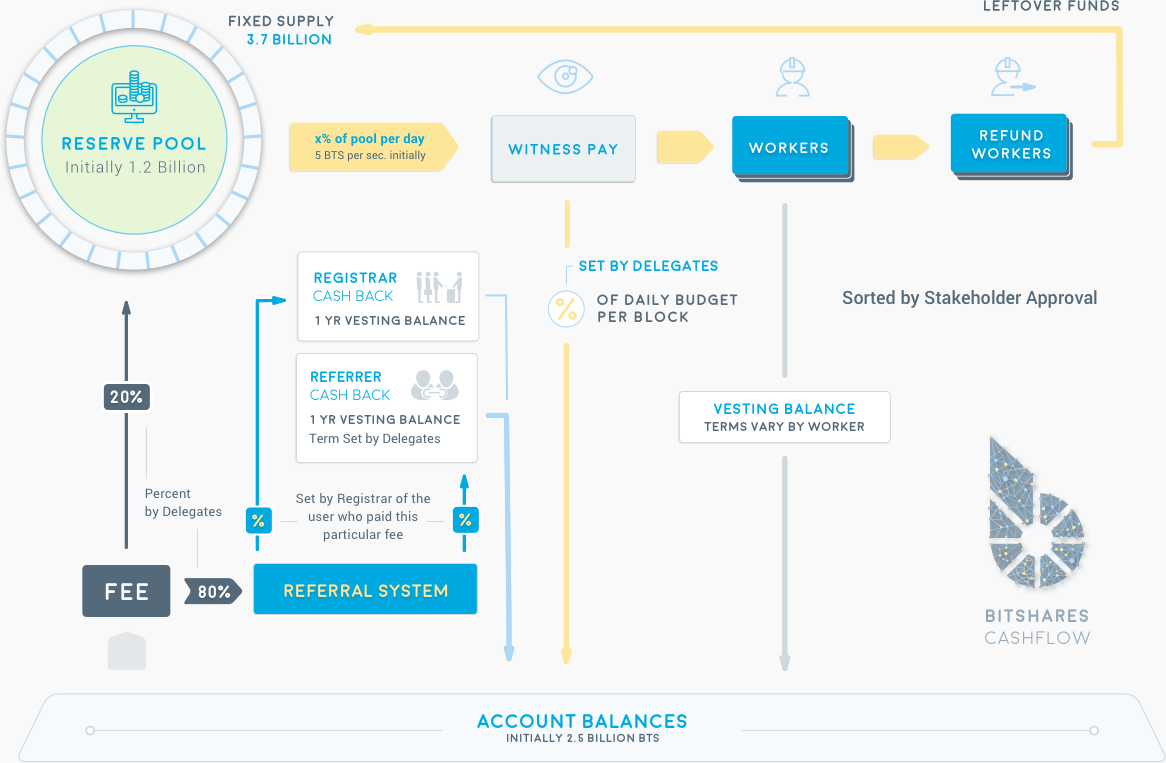
\includegraphics[width=.8\linewidth]{figures/cashflow.png}
 \caption{Cash flow of BitShares 2.0}
 \label{fig:cashflow}
\end{figure*}

%% Revenue
Revenue streams are essentially caused by fees that have to be payed when using
the DACs products, such as market pegged assets, user-issued assets, or the
decentralized exchange~\cite{bts:financial}. These fees are variable, can be
changed by shareholder approval and include
\begin{inparaenum}[(a)]
 \item transfers,
 \item order operations,
 \item account operations,
 \item asset operations,
 \item witness creations
 \item proposal operations
 \item withdraw permission operations
 \item committee member operations,
 \item worker creation,
\end{inparaenum}
and more.

%% Costs
In contrast to bitcoin, where newly created coins in each block are distributed
solely among countless miners that immensely overpay for the network
security~\cite{ltb:dac}, the BitShares ecosystem achieves a better security at
lower costs by means of an adjustable number of approved and trusted witnesses
in DPOS. Additionally, the BitShares ecosystem has the capability to pay for
its own development through budget items. Both, the payment for witnesses, as
well as the budget items are required to be approved by the shareholders.

As an example, an entrepreneur may approach the shareholders and offer to
launch a business in the BitShares space that would greatly benefit the
ecosystem. If he succeeds and convinces the shareholders to vote for and not
against his plan, he could get an initial funding by the DAC.

Another use-case would be the improvement of the blockchain's protocol. A
developer could propose a change or extension of the existing software
implementation and be payed by the DAC to do so (after shareholder approval).
Hence, as long as the average shareholders acts rational, the BitShares
blockchain can be seen as a self-funded but profitable business


\subsection    { Memberships                       } Accounts in BitShares are separated into three groups. We decided to give users
the option to upgrade their accounts into a VIP-like status if they desire and
profit from reduced fees and additional features.

A \emph{regular} account is a \emph{non-member}.

\emph{Lifetime Members} get a percentage cashback on every transaction fee they
pay and qualify to earn referral income (see below) from users they register
with or refer to the network. A Lifetime membership is associated with a
certain one-time fee that is defined by the committee and qualifies for reduced
transaction fees.

If a lifetime membership is too much you can still get the same cashback for
the next year by becoming an annual subscriber for a smaller one-time fee which
lasts for only one year and qualifies for reduced transactions fee during that
time.

\subsection    { Referral Program                  } Every time an account you referred pays a transaction fee, that fee is divided
among several different accounts. The network takes a cut, and the Lifetime
Member who referred the account gets a cut.

The registrar is the account that paid the transaction fee to register the
account with the network. The registrar gets to decide how to divide the
remaining fee between themselves and their own affiliate.

Fees paid are only divided among the network, referrers, and registrars once
every maintenance interval. The paid fees are divided among tow or three
parties, depending on the parameter $d$ that can be set by the registrar:

\begin{align}
 \text{total fee} &= \text{network fee} (20\%) \notag\\
                  &\quad+ \text{registrar} (80\%\cdot(100\%-d\%)) \\
                  &\quad+ \text{referrer} (80\%\cdot(d\%)) \notag
\end{align}

Most fees are made available immediately, but fees over the vesting threshold
(such as those paid to upgrade your membership or register a premium account
name) must vest for some days as defined by the committee.
 

\section       { Architecture of BitShares         } Before describing how BitShares can be used to secure financial freedom, we
first discuss the technical specifications briefly. Among these is the public
ledger (also referred to as \emph{the blockchain}), the peer-to-peer network,
the distributed consensus finding mechanism and the system parameters available
to BitShares. We will furthermore describe the use of objects to implement
different entities on the blockchain.
 
\subsection    { Public Ledger                     } \newcommand*\justify{%
  \fontdimen2\font=0.4em% interword space
  \fontdimen3\font=0.2em% interword stretch
  \fontdimen4\font=0.1em% interword shrink
  \fontdimen7\font=0.1em% extra space
  \hyphenchar\font=`\-% allowing hyphenation
}

As in other crypto-currencies, the public ledger of BitShares is built and
stored in a linked series of blocks, known as a blockchain.

The ledger provides a permanent record of transactions that have taken place,
and also establishes an order in which transactions have occurred. Hence, every
\emph{content} of the blockchain can be assigned an permanent and unique
identifier in form of a scalar number.

Every full node in the BitShares network stores a full copy of this blockchain
and can verify its validity and the evaluate new blocks.

Every block contains
\begin{itemize}
 \item a reference to the previous block,
 \item a timestamp,
 \item a hash of a secret,
 \item the secret of the previous hash,
 \item a set of transactions, and
 \item a signature by the block producing authority
\end{itemize}

As will be discussed in \cref{sec:consensus}, the consensus mechanism allows
for synchronous block production with constant block confirmation times, e.g.,
one block every \SI{5}{\second}.

Since the blocks mainly embrace customer transactions but has to perform time
intensive tasks, or execute rare events from time to time, some actions such as
reenumeration of blockchain-based votes and rare events such as newly
registered block producers (witnesses) are carried out more rarely but still on
a frequent so called \emph{maintenance interval}.

% The following parameters are associated with the blockchain operations and are
% subject to shareholder consensus:
% %
% \begin{description}[leftmargin=4em,style=nextline]
%  \item[\texttt{block-interval}] time in seconds between blocks
%  \item[\texttt{maintenance-interval}] time in seconds for a maintenance
%                                       interval to evaluate more time-consuming tasks
%  \item[\texttt{maximum-transaction-size}] maximum size of a transaction in bytes
%  \item[\texttt{maximum-block-size}] maximum size of a block in bytes
%  \item[\texttt{maximum-witness-count}] number of witnesses allowed to actively
%                                        produce blocks
%  \item[\texttt{maximum-committee-count}] maximum amount of committee members to
%                                          take into account for parameter definition.
% \end{description}

 
\subsection    { Irreversibility of Transactions   } Historically we have stated that a blockchain becomes irreversible after one
round of block production with greater than 51\% participation. It turns out
that this metric is too fuzzy because of noise in how witnesses are ordered. In
an effort to provide stronger/absolute guarantees a new metric has been derived
that determines the exact point at which a particular block becomes
\emph{irreversible}. The algorithm to define the metric goes as follows:

Sort $N$ witnesses by the last block number they signed, then take the highest
block number that is lower than 66\% of all other witnesses. This will indicate
that said block has been confirmed by 66\% of all witnesses and is clearly
irreversible.

This particular metric is dynamic and can respond to changes in the order of
witnesses and is immune to situations where the network fragments into more
than two pieces. In the event of a major disruption users are guaranteed that
no block older than that number can ever be undone. 

If we had only 17 witnesses and 3 second block confirmation interval, then this
will take an average of 34 seconds. If we had 101 witnesses and 3 second blocks
then this will take an average of 3.3 minutes for block to be
\emph{irreversible},

Having this metric is important to give everyone in the network peace of mind
in the unlikely event that a software bug or network issue causes all witnesses
to fall out of sync and gives a clear measure of when they are considered back
in sync.

Anyone accepting transactions as final prior to the most recent irreversible
block is choosing to take some extra risk on their transaction.

\subsection    { Low Latency Peer-to-Peer Network  } The peer-to-peer network distributes the full blockchain database across the
world. It consists of public and private nodes as well as seed nodes that are
used for initial connection to the peer-to-peer network. Anybody may connect to
any known node and download the current global and unique state (i.e. the
blockchain).

Once a node is in sync with the peer-to-peer network it received and applies
newly created blocks, and assists new network nodes by further distribution of
the blockchain. Additionally, new blocks are broadcast to all connected nodes.

Furthermore, network nodes receive transaction from participants and forward
them to the rest of the network until they reach the witness that is in charge
of constructing the next block. Hence, new transaction broadcasts do not
necessarily need to reach all nodes.

On reception of new transactions by a witness node, the witness validates its
operations and advances the blockchain state by one block containing that
transaction (and possibly many more).

If a node does not receive a block, it will request it when it receives the
next block and realizes it missed one. If a witness did not receive its
previous block at the time it is supposed to construct its block, the previous
block will be marked as \emph{missed} and a reference to the block before the
previous block will be used instead. A more detailed description about the
distributed consensus mechanism as well as a discussion how blockchain forking
is prevented during attacks is given in a separate paper~\cite{}. % FIXME link dpos paper
 
\subsection    { Distributed Consensus Mechanism   } \label{sec:consensus}

Consensus is the mechanism by which a subset of people decide upon unitary
rational action. The process of consensus decision-making allows for all
participants to consent upon a resolution of action even if not the favored
course of action for each individual participant. Bitcoin was the first system
to integrate a fully decentralized consensus method with the modern technology
of the internet and peer-to-peer networks in order to more efficiently
facilitate the transfer of value through electronic communication. The
proof-of-work structure that secures and maintains the Bitcoin network is one
manner of organizing individuals who do not necessarily trust one another to
act in the best interest of all participants of the network.

It is of importance to distinguish a democratic voting process in which every
citizen of a community has one and only one vote from a distributed consensus
mechanism in cryptocurrencies hand over voting power either in relation to
hashing power (e.g. proof-of-work) or on a per stake basis (e.g.
proof-of-stake). In both cases, those that invest in the required
infrastructure to increase their voting percentage (i.e. by buying mining
hardware or stake) act as shareholder in a distributed community.

The BitShares community employs \emph{Delegated Proof-of-Stake} (DPOS) in order
to find efficient solutions to distributed consensus decision making.  DPOS
attempts to solve the problems of both Bitcoin's traditional proof-of-work
system, and the proof-of-stake system of Peercoin and NXT by implementing a
layer of technological democracy to offset the negative effects of
centralization. For historical reasons, the technology is still called
\emph{delegated} proof-of-stake even though what have been delegates in
BitShares 1.0 are now so called \emph{witnesses}.

In DPOS set of $N$ witnesses (formerly known as \emph{delegates}) sign the
blocks and are voted on by those using the network with every transaction that
gets made. By using a decentralized voting process, DPOS is by design more
democratic than comparable systems. Rather than eliminating the need for trust
all together, DPOS has safeguards in place the ensure that those trusted with
signing blocks on behalf of the network are doing so correctly and without
bias. A more detailed description about the distributed consensus mechanism as
well as a discussion how blockchain forking is prevented during attacks is
given in a separate paper~\cite{}. % FIXME link dpos paper

Additionally, each block signed must have a verification that the block
before it was signed by a trusted node. DPOS eliminates the need to wait until
a certain number of untrusted nodes have verified a transaction before it can
be confirmed.

This reduced need for confirmation produces an increase in speed of transaction
times. By intentionally placing trust with the most trustworthy of potential
block signers, as decided by the network, no artificial encumbrance need be
imposed to slow down the block signing process. DPOS allows for many more
transactions to be included in a block than either proof of work or proof of
stake systems.

In a delegated proof-of-stake system, centralization still occurs, but it is
controlled. Unlike other methods of securing cryptocurrency networks, every
client in a DPOS system has the ability to decide who is trusted rather than
trust concentrating in the hands of those with the most resources. DPOS allows
the network to reap some of the major advantages of centralization, while still
maintaining some calculated measure of decentralization. Furthermore, once a
delegates has reached approval by shareholders, surpasses the threshold of the
most $N$ active witnesses, and, hence, is elected to actively participate in
the block production procedure, its power is \emph{equivalent} to all other
active witnesses. This system is enforced by a fair election process where
anyone could potentially become a delegated representative (witness) of the
majority of users.

Please note that DPOS has a recommended $1-2$ block confirmation versus
bitcoin's 6 block recommendation. DPOS is much more resistant against forks for
the following reasons:
\begin{itemize}
\item When a fork is produced it is
      very likely that all delegates have seen and processed your transaction and
      thus no alternative transactions can be broadcast and the next delegate is
      almost certain to include your transaction.  All delegates are much more
      trusted than miners.
\item The probability of a fork after a block has been produced is very low (<
      0.01\%) where as Bitcoin has 25 orphans in the last 22 days (about 1 per day in
      Dec 3,2014) which translates into 0.7\% of blocks are orphaned.
\item On normal operations, DPOS achieves a 100\% witness participation rate and when
      we are less than that it is more often because a delegate went offline and didn't
      produce a block than because they produced a fork. 
\item In BitShares 1.0 forks have almost always been resolved within 30 seconds. 
\end{itemize}

Assuming a 10 second block interval, Bitshares is mathematically over 70x less
likely to orphan after 1 block than Bitcoin after 1 block (10 minutes). After 3
blocks (30 seconds) any random orphan will have been resolved and the
probability of alternative chains is much lower than the 0.000001\% of Bitcoin.
By the time Bitcoin gets to .7\% orphan probability, BitShares has 60 blocks
which would have a probability of being orphaned of less than $10^{-120}$.

% FIXME: review these numbers
 
\subsection    { Operations                        } Similar to most crypto-currencies, there is a set of predefined operations that
can be performed on the blockchain. In contrast to Bitcoin, which uses a
technique called \emph{script} to describe operations that shall be performed
in a programmatic way using \emph{OP} codes, the BitShares network has a
predefined (but extensible) set of operations that a user may perform.

All operations end up on the blockchain eventually. Once they are validated and
confirmed by a witness by being included into a block, they are \emph{executed}
and update the state of the blockchain accordingly.

The release version of BitShares 2.0 comes with 
\begin{inparaenum}[(a)]
 \item transfer ops,
 \item trading order ops,
 \item account ops,
 \item asset ops,
 \item witness ops,
 \item committee ops,
 \item worker ops, and
 \item vesting ops,
\end{inparaenum}
However, since BitShares allows for shareholder approved, live protocol
upgrades, the set of operations can be extended and modified. 
% FIXME do we allows for modifications of existing ops?

On the blockchain level, each operation is assigned an individual \emph{id}
with a custom set of parameters for performance and latency reasons.

% FIXME example(?)
 
\subsection    { Transactions                      } Having defined \emph{operations}, we can now put these into a \emph{list of
operations} and construct a \emph{transaction}.

\begin{verbatim}
{
   "ref_block_num": ...,
   "ref_block_prefix": ...,
   "expiration": [...],
   "extensions": [...],
   "operations": [...],
   "signatures": [...],
}
\end{verbatim}

In addition to its operations, a transaction also consists of 
\begin{inparaenum}[(a)]
 \item an expiration date,
 \item a reference block number,
 \item a reference block prefix,
 \item a set of extensions, and
 \item a set of signatures to authorize each operation.
\end{inparaenum}

Each node (including witnesses) verifies that all requires signatures to
perform the given operations are present and valid prior to propagating the
transactions to the rest of the network and hence to the witness node
constructing the next block. If the transaction is included into a block it is
considered \emph{finally valid} or \emph{executed}.
 
\subsection    { Proposed Transactions             } Additionally, the Graphene technology allows users to propose a transaction
which requires approval of multiple accounts in order to execute.
These transactions are only partially valid and do not \emph{execute} until
they are completely valid.

The user proposes a transaction, then signatory accounts add or remove their
approvals from this operation. When a sufficient number of approvals have been
granted, the operations in the proposal are used to create a virtual
transaction which is subsequently evaluated. Even if the transaction fails, the
proposal will be kept until the expiration time, at which point, if sufficient
approval is granted, the transaction will be evaluated a final time. This
allows transactions which will not execute successfully until a given time to
still be executed through the proposal mechanism. The first time the proposed
transaction succeeds, the proposal will be regarded as resolved, and all future
updates will be invalid.

The common use-case would be similar to so called \emph{multi-signature}
transactions which must be signed by two parties. Classical crypto currencies
had the issue that such \emph{proposed} transaction had to be communicated on
separated channels until all required signatures have been collected.
With BitShares, it is no possible to propose a transaction on the blockchain
and have the required signatures be added by the respective parties.

The proposal system in combination with corporate accounts allows for
arbitrarily complex or recursively nested authorities. If a recursive authority
(i.e. an authority which requires approval of \emph{nested} authorities on other
accounts) is required for a proposal, then a second proposal can be used to
grant the nested authority's approval. That is, a second proposal can be
created which, when sufficiently approved, adds the approval of a nested
authority to the first proposal. This multiple-proposal scheme can be used to
acquire approval for an arbitrarily deep authority tree.

%\subsection    { Objects                           } Speaking abstractly, the BitShares blockchain does not distinguish between
assets, account, or operations. These terms do only exist outside the
blockchain. Instead, the blockchain deals with \emph{contextual objects} that
are associated with a given set of features, permissions, etc.

Hence, on the BitShares blockchains there are no addresses similar to Bitcoin,
but objects identified by a unique \emph{id}, a \emph{type} and a \emph{space}
in the form:

\begin{verbatim}
   space.type.id
\end{verbatim}

The reserved \emph{space} are
\begin{verbatim}
   enum reserved_spaces {
      relative_protocol_ids = 0,
      protocol_ids          = 1,
      implementation_ids    = 2
   };
\end{verbatim}

As an example, we have the following objects:
\begin{description}[leftmargin=4em,style=nextline]
 \item[1.2.15]   15th blockchain account
 \item[1.6.105]  105th blockchain witness
 \item[1.14.7]   7th blockchain worker proposal
 \item[2.1.0]    wallet dynamic global properties
 \item[2.3.8]    8th asset
\end{description}

A programmatic description of all fields can be found in the sources.
 

\section       { Discussion                        } The inherent problems of Bitcoin and other Cryptocurrencies

    Slow transactions per second (TPS) when compared to major payment processors like VISA. (7 TPS with Bitcoin vs 10,000 TPS with VISA)
    Addresses are machine readable, not human readable. As a result ~5\% of BTC have been irrevocably lost.
    Transactions are not anonymous.
    Security of the network consumes between \$500 million and \$1 billion annually, depending on the Bitcoin market capitalization.
    Control of the network is proportional to hashing power, not proportional to one's Bitcoin holdings.
    Centralization of hashing power can come under the control of a single mining pool.
    High price volatility. This is the biggest deterrent when it comes to adoption as a major currency.

How BitShares solves these issues

    BitShares Uses block rewards to directly fund development and marketing as opposed to spending on mining equipment and electricity.
    DPOS reduces block production to 10 seconds. Since computational resources are used for the purpose of transaction propagation and confirmation, rather than wasteful computational work, DPOS blockchains can scale to the transaction load of visa.
    BitShares uses accounts that can be registered on the blockchain. Users no longer need to send money to an alphanumeric string that can be copied incorrectly. Rather, money can be sent as easily as sending an email, and in the same fashion. It is very difficult to send to a wrong account. You can still send to public keys but its unnecessary and adds little advantage.
    Name registration allows for the identification of who transactions are are originating with with no need to manually create a contact account for a given address.
    Transactions contain a memo field that allow users to describe the nature of the transaction or broadcast secure messages about the price of the current transaction fee.
    BitShares uses TITAN, which automates the creation of stealth address using an accounts registered public key. There is no longer a need for mixing or "master nodes." Transactions are more anonymous than Bitcoin, for example, with no additional work needed from the user.
    BitShares is a 100\% proof-of-stake system. This means it is a lot more efficient (cost per security) than proof-of-work and therefore does not have to dilute stakeholders/coinholders (there is a ~10\% dilution of Bitcoin-holders per year with Bitcoin and lowering this dilution would mean to lower the security). Proof of stake does not depend on hash rate for security.
    BitShares is a bank and decentralized exchange allowing people to hold deposits in whatever asset they choose. This system allows investors with a higher risk tolerance to collateralize and trade virtual assets. Users who simply want to use crypto-currencies as a stable medium of exchange can do so without risk, due to the volatility of the network's main equity/currency. For example, if a user were to put \$100 in the network, the deposit is always redeemable for \$100 worth of BitShares, as a result of the free market peg of bitUSD to real USD.
    The cost of securing the network is merely a fraction of all transaction fees accumulated by the network.
    Delegates compete for votes and the top 101 delegates produce blocks. The job of a basic delegate is simple: include as many valid transactions in your given block as possible and sign a single block. If a delegate signs multiple blocks they are immediately fired. If a delegate blocks transactions, they will be voted out of office. Each round delegates are randomly assigned a block to produce, thereby making it that much harder to coordinate a sustained attack on the network - without 51\% of the shares.
    Shareholder votes are proportionate to the relative number of shares they own. The DAC is completely shareholder run.
    Now people can be hired by the blockchain. By running a delegate with a higher than basic payrate, a person can attempt to be voted into a position on the blockchain. Where coins like Bitcoin dilute to pay for network security, BitShares takes these fees and directs them towards continual improvement of the network and community. This helps insure BitShares will stay competitive in its featureset.

 

\section       { Conclusion                        } The properties and features mentioned in this paper make it clear that the
BitShares DAC is well-prepared for its own features. It was shown that, due to
on-blockchain voting, a decentralized development and funding can be achieved.
The consensus mechanism DPOS reaches a trade-off between efficiency and
required trust while maintaining better decentralization than almost every other
blockchain consensus scheme.
 

% acknowledgment @ cass!!

\bibliographystyle{IEEEtran}
\bibliography{literature}
%\nocite{*}
\end{document}
